\documentclass[11pt]{article}

\usepackage{amsmath}
\usepackage{amssymb}
\usepackage{textcomp}
\usepackage{bbm}
\usepackage{graphicx}
\graphicspath{ {./} }
\usepackage{wrapfig}
\usepackage[top=0.8in, bottom=0.8in, left=0.8in, right=0.8in]{geometry}
% Add other packages here 


% Put your group number and names in the author field %
\title{\bf Exercise 5: An Auctioning Agent for the Pickup and Delivery Problem}
\author{Group \textnumero : 90  Kyle Gerard, Yann Bolliger}


\begin{document}
  \maketitle

  \section{Bidding strategy}

  % Do you consider the probability distribution of the tasks in defining your
  % strategy? How do you speculate about the future tasks that might be auctions?
  %
  % How do you use the feedback from the previous auctions to derive information
  % about the other competitors?
  %
  % How do you combine all the information from the probability distribution of the
  % tasks, the history and the planner to compute bids?

  \subsection{General strategy}

  For the auction agent we implemented a bidding strategy on top of our stochastic
  local search solution from the last assignment. We tweaked the search's
  parameters in order to have faster convergence but otherwise the algorithm
  remains unchanged. The bidding strategy we opted for follows a simple,
  aggressive but powerful concept:

  \begin{quotation}
    Take the first tasks at loss and subsequently enjoy lower marginal costs!
  \end{quotation}

  All our design choices rely on this idea. If the vehicle already travels to
  cities on the map then -- assuming maps dense enough, like the ones we were
  given -- it is likely that part of a new parcel's journey is already on the
  vehicles path. If this is the case then this part of the parcel's delivery is
  already paid for and we can offer it at a lower price than the cost.

  At each bidding round we compute two values that we will discuss in the
  following subsection. Combined with some bookkeeping about won tasks and
  gains, we calculate the final bid. This calculation is different on depending
  three phases the agent can be in and that are explained below.


  \subsection{Marginal cost and expected gains}

  Upon receiving a task to bid for, we let the planner schedule a plan based on
  the solution of the last iteration but with the additional task that is offered.
  The cost of this new schedule minus the cost of the previous one yields the
  marginal cost. This is the cost that our schedule incurs from delivering the
  additional task. However, this does not take into account the possibility of
  future tasks. If for example the next auctioned task has the same route as
  the current one, then -- provided enough capacity -- we could deliver the next
  task for free.

  To account for future tasks we introduce the \textbf{expected maximum gain}
  $\mathbb{E}[maxGain]$ of a schedule. It measures how much more gains could be
  made if all our vehicles $v \in \mathcal{V}$ were full at each move $m \in
  \mathcal{M}$.
  \begin{eqnarray*}
    \mathbb{E}[maxGain] &=&
    \sum_{v \in \mathcal{V}}
    \sum_{m \in \mathcal{M}}
    length(m) \cdot cost(v) \cdot
    loadFactor\cdot
    \mathbb{E}[remainingTasks]
    \\
    loadFactor &=& \max\left(0, \min\left(
    \frac{\mathbb{E}[load(v, m)] - load(v, m)}{capacity(v)},
    1 \right)\right)
    \\
    \mathbb{E}[load(v, m)] &=&
    \sum_{c_p \in \mathcal{C}} \sum_{c_d \in \mathcal{C}}
    \mathbb{P}(task(c_p \rightarrow c_d))
    \cdot \mathbb{E}[weight(c_p, c_d)] \cdot
    \mathbbm{1}\{task(c_p \rightarrow c_d) \text{ contains } m\}
  \end{eqnarray*}

  Where $load(v, m)$ is the current load of vehicle $v$ when performing move $m$.
  For better understanding, let us look at a toy example. Consider one vehicle
  with $capacity(v) = 2$ and cities $A \leftrightarrow B \leftrightarrow C$. If
  the vehicle is initially at $A$ and already delivers a task of weight 1 from $B
  \rightarrow C$ then it could still take tasks with weight 2 from $A \rightarrow
  B$ and weight 1 from $B \rightarrow C$. But this is only true if there are
  future auctions where such tasks might appear. This is captured by
  $\mathbb{E}[load(v, m)]$ which takes into account the probability distribution
  of tasks and their expected weights from \texttt{TaskDistribution} as well as
  the guessed $\mathbb{E}[remainingTasks]$. The guess is a simple decreasing
  $\log$ function based on the assumption that there will usually be between 10
  and 60 tasks in total.

  As with the marginal cost it is now possible to calculate the marginal expected
  gain at each round by subtracting the previous expected gain. If this quantity
  is large it indicates that taking the offered task will augment our
  possibilities of making profit in the future. If on the other hand it is small
  or even negative it shows us that auctioned task does not bring us any benefit
  in future auctions and it is therefore less valuable to us. In that sense the
  marginal expected gain can be seen as a \textit{utility function} that estimates
  how a task will change our chances of profit in the future.

  \subsection{Bidding phases}

  With those computations in place we calculate our bids based on three states.
  In all of them we put a lower bound $l$ on the bids that is some fraction of the
  path's cost. This is a price that nobody can beat but it prevents the agent from
  bidding 0 when the marginal cost is 0.

  \begin{itemize}

    \item

    \textbf{Phase 1}: At the beginning we want to take all the tasks. Therefore we
    bid at deficital prices. The amount of deficit we make depends on how much
    utility the task will bring us in the future. We lower the bid for high
    utilities ($\alpha$ was determined experimentally and set to 0.1):
    $$
    bid = \max(l, marginalCost - marginalExpectedGain \cdot \alpha)
    $$

    \item

    \textbf{Phase 2}: Once the number of won tasks plus the number of auctioned
    tasks is larger than 6, we go into the second phase. This phase aims to catch
    up the deficits that were made in phase 1. The idea is to always be profitable
    after 10 rounds. Therefore the bids in this phase take into account the
    current deficit $d$ of the agent:
    $$
    bid = \max(l, marginalCost + d/\max(1, 10 - round))
    $$

    \item

    \textbf{Phase 3}: When the agent is profitable again it transitions to the
    last phase. Similarly as in phase 1, the bids are determined by the utility of
    the offered task but unlike before they are never deficital.
    ($\beta$ was determined experimentally and set to 0.2):
    $$
    bid = \max(l, marginalCost + \max(1, 1 - marginalExpectedGain \cdot \beta)
    $$


  \end{itemize}


  \section{Results}

  % in this section, you describe several results from the experiments with your
  % auctioning agent

  \subsection{Experiment 1: Comparisons with dummy agents}

  % in this experiment you observe how the results depends on the number of tasks
  % auctioned. You compare with some dummy agents and potentially several versions
  % of your agent (with different internal parameter values).

  \subsubsection{Setting}

  % You describe how you perform the experiment, the environment and description
  % of the agents you compare with
  
  We use the default configuration file \texttt{auction.xml} with 60 tasks and
  run two auctions (5 seconds bid time, 15 seconds plan time). In the first
  auction, our agent competes against our ``dummy'' agent which always bids:
  $marginalCost + 1$. In the second auction, our agent competes against our
  ``random dummy'' agent which always bids: $marginalCost \cdot
  (\mathtt{Math.random()} \cdot 0.5 + 1)$. For all three agents, the marginal
  cost is calculated using the same stochastic local search algorithm.

  \newpage

  \subsubsection{Observations}
  
    \begin{wrapfigure}{R}{0.7\textwidth}
      \vspace{-20pt}
    \label{fig1}
 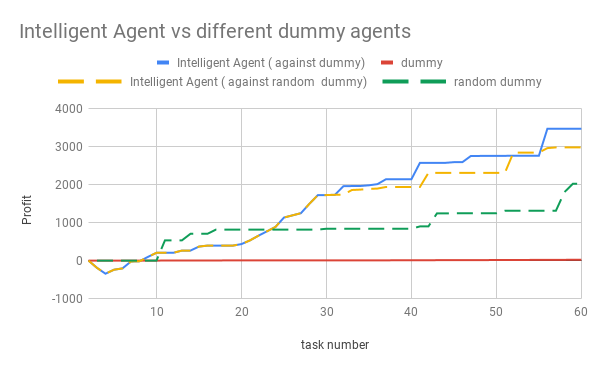
\includegraphics[width=0.7\textwidth]{dummy.png}
 \vspace{-20pt}
 \end{wrapfigure} 
  
  In the plot \ref{fig1} we observe that our agent wins the auction against both dummy
  agents at the end of the 60 tasks. However, because the first tasks are taken
  at loss and because the ``random dummy'' agent is lucky on task 10 and gains
  500 profit, our agent would have lost had there been less than 23 tasks. 
  

  Out of the numerous runs we did against the random agent, our agent almost
  always won the auction after 10-13 tasks. Moreover, we know that all auctions
  will have at least 10 tasks and that random agents can get lucky against any
  algorithm so we decided that winning most of the time was sufficient.

  \subsection{Experiment 2: Varying the discount factor $\alpha$ in phase 1 of
  our strategy}
  
  % Other experiments you would like to present (for example, varying the internal
  % parameter values)

  \subsubsection{Setting}
  
  We used the default configuration file \texttt{auction.xml} with 30 auctioned
  tasks (5 seconds bid time, 15 seconds plan time) and ran multiple auctions
  while varying the discount factor $\alpha$ in phase 1 of our bidding strategy.
  Our agent competed against our ``dummy'' agent which always bids:
  $marginalCost + 1$.

  \subsubsection{Observations}

\begin{wrapfigure}{R}{0.7\textwidth}
  \vspace{-20pt}
    \label{fig2}
 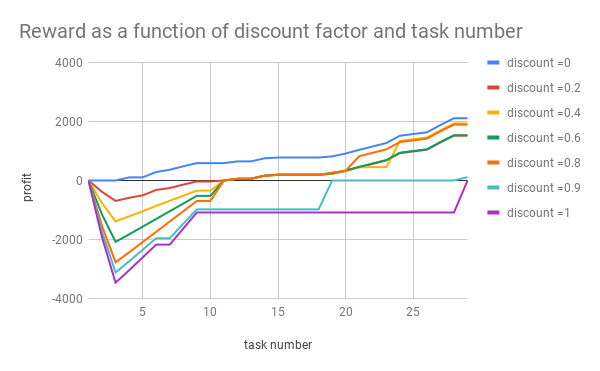
\includegraphics[width=0.7\textwidth]{discount.png}
 \vspace{-20pt}
 \end{wrapfigure} 
  

  In the plot \ref{fig2} we see how our agent's losses increase during phase 1 of our
  strategy as a function of the discount factor $\alpha$. We remark that up to
  the discount factor of $\alpha = 0.8$ our agent is able to recover its losses
  by the 10th task. With a larger $\alpha$ however, we see that the agent looses
  most of its bids because they are too high, trying to regain its high losses
  from before. 
  
  Our conclusion from this experiment is that our strategy is
  functional with $\alpha \leq 0.8$. Indeed, whatever losses we incur in phase 1
  of our strategy, we are later able to regain them because of lower marginal
  costs due to having a lot more tasks than our opponent.

\end{document}
